\documentclass{standalone}
\usepackage{tikz}
\usetikzlibrary{patterns}

\begin{document}
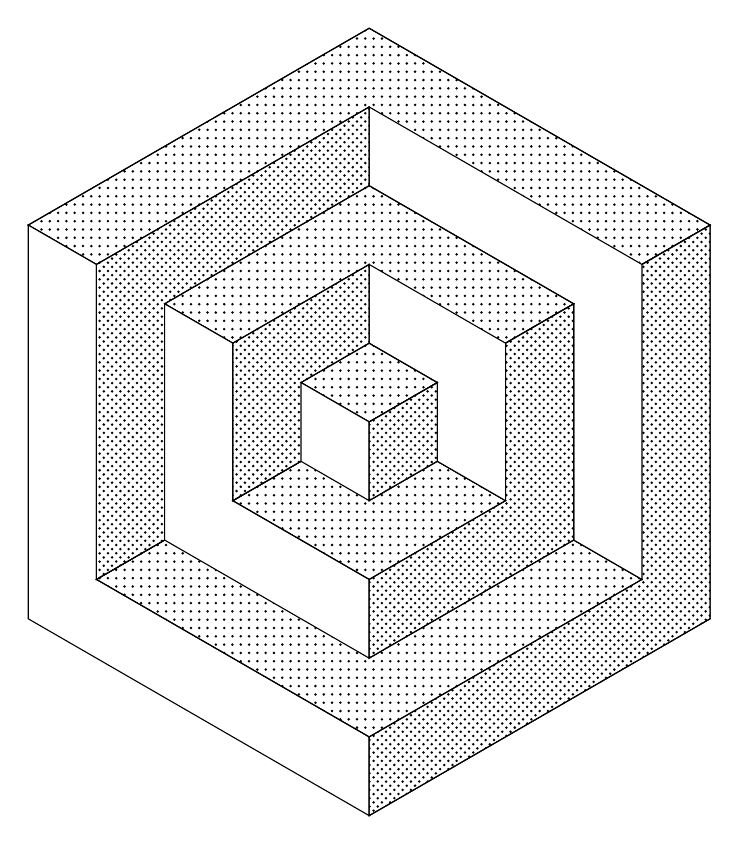
\begin{tikzpicture}[rotate=210]
  \foreach \scale in {5,...,1} {
    \draw[fill=white] (0,0)--(0+180*\scale:\scale)--(60+180*\scale:\scale)--(120+180*\scale:\scale)--	cycle;
    \draw[fill,pattern=dots] (0,0)--(0+180*\scale:\scale)--(60+180*\scale:\scale)--(120+180*\scale:\scale)--cycle;

    \draw[fill=white] (0,0)--(120+180*\scale:\scale)--(180+180*\scale:\scale)--(240+180*\scale:\scale)--cycle;

    \draw[fill=white] (0,0)--(240+180*\scale:\scale)--(300+180*\scale:\scale)--(0+180*\scale:\scale)--cycle;
    \draw[fill,pattern=crosshatch dots] (0,0)--(240+180*\scale:\scale)--(300+180*\scale:\scale)--(0+180*\scale:\scale)--cycle;
  }
\end{tikzpicture}
\end{document}
